%This work is licensed under the Creative Commons Attribution-NonCommercial-NoDerivs 3.0 United States License. To view a copy of this license, visit http://creativecommons.org/licenses/by-nc-nd/3.0/us/ or send a letter to Creative Commons, 444 Castro Street, Suite 900, Mountain View, California, 94041, USA.

\section{Two-photon Assisted Thermionic Photoemission} \label{sec:two_photon}

\begin{figure}
  \centering
  \begin{tikzpicture}
  %% \begin{tikzpicture}[gnuplot]
%% generated with GNUPLOT 4.6p0 (Lua 5.1; terminal rev. 99, script rev. 100)
%% Wed 14 Nov 2012 02:16:58 PM CST
\path (0.000,0.000) rectangle (12.500,8.750);
\gpcolor{color=gp lt color border}
\gpsetlinetype{gp lt border}
\gpsetlinewidth{1.00}
\draw[gp path] (1.504,0.985)--(1.684,0.985);
\draw[gp path] (11.485,0.985)--(11.305,0.985);
\node[gp node right] at (1.320,0.985) { 450};
\draw[gp path] (1.504,2.042)--(1.684,2.042);
\draw[gp path] (11.485,2.042)--(11.305,2.042);
\node[gp node right] at (1.320,2.042) { 500};
\draw[gp path] (1.504,3.098)--(1.684,3.098);
\draw[gp path] (11.485,3.098)--(11.305,3.098);
\node[gp node right] at (1.320,3.098) { 550};
\draw[gp path] (1.504,4.155)--(1.684,4.155);
\draw[gp path] (11.485,4.155)--(11.305,4.155);
\node[gp node right] at (1.320,4.155) { 600};
\draw[gp path] (1.504,5.211)--(1.684,5.211);
\draw[gp path] (11.485,5.211)--(11.305,5.211);
\node[gp node right] at (1.320,5.211) { 650};
\draw[gp path] (1.504,6.268)--(1.684,6.268);
\draw[gp path] (11.485,6.268)--(11.305,6.268);
\node[gp node right] at (1.320,6.268) { 700};
\draw[gp path] (1.504,7.324)--(1.684,7.324);
\draw[gp path] (11.485,7.324)--(11.305,7.324);
\node[gp node right] at (1.320,7.324) { 750};
\draw[gp path] (1.504,8.381)--(1.684,8.381);
\draw[gp path] (11.485,8.381)--(11.305,8.381);
\node[gp node right] at (1.320,8.381) { 800};
\draw[gp path] (1.504,0.985)--(1.504,1.165);
\draw[gp path] (1.504,8.381)--(1.504,8.201);
\node[gp node center] at (1.504,0.677) { 0};
\draw[gp path] (2.920,0.985)--(2.920,1.165);
\draw[gp path] (2.920,8.381)--(2.920,8.201);
\node[gp node center] at (2.920,0.677) { 2};
\draw[gp path] (4.335,0.985)--(4.335,1.165);
\draw[gp path] (4.335,8.381)--(4.335,8.201);
\node[gp node center] at (4.335,0.677) { 4};
\draw[gp path] (5.751,0.985)--(5.751,1.165);
\draw[gp path] (5.751,8.381)--(5.751,8.201);
\node[gp node center] at (5.751,0.677) { 6};
\draw[gp path] (7.167,0.985)--(7.167,1.165);
\draw[gp path] (7.167,8.381)--(7.167,8.201);
\node[gp node center] at (7.167,0.677) { 8};
\draw[gp path] (8.583,0.985)--(8.583,1.165);
\draw[gp path] (8.583,8.381)--(8.583,8.201);
\node[gp node center] at (8.583,0.677) { 10};
\draw[gp path] (9.998,0.985)--(9.998,1.165);
\draw[gp path] (9.998,8.381)--(9.998,8.201);
\node[gp node center] at (9.998,0.677) { 12};
\draw[gp path] (11.414,0.985)--(11.414,1.165);
\draw[gp path] (11.414,8.381)--(11.414,8.201);
\node[gp node center] at (11.414,0.677) { 14};
\draw[gp path] (1.504,8.381)--(1.504,0.985)--(11.485,0.985)--(11.485,8.381)--cycle;
\node[gp node center,rotate=-270] at (0.246,4.683) {HWe$^{-1}$M Beam Size($\mu$m)};
\node[gp node center,rotate=-270] at (11.792,4.683) {Electron Yield (a.u.)};
\node[gp node center] at (6.494,0.215) {Incident Laser Pulse Energy (nJ)};
\gpcolor{color=gp lt color 0}
\gpsetlinetype{gp lt plot 0}
\draw[gp path] (1.504,1.217)--(2.495,2.063)--(3.486,2.718)--(4.477,3.267)--(5.468,3.732)%
  --(6.459,4.155)--(7.450,4.535)--(8.441,4.873)--(9.432,5.190)--(10.423,5.465)--(11.414,5.761);
\gpcolor{rgb color={1.000,0.000,0.000}}
\gpsetlinetype{gp lt plot 1}
\draw[gp path] (1.504,1.196)--(2.495,2.232)--(3.486,2.992)--(4.477,3.605)--(5.468,4.134)%
  --(6.459,4.577)--(7.450,5.000)--(8.441,5.359)--(9.432,5.718)--(10.423,6.035)--(11.414,6.331);
\draw[gp path] (1.504,1.260)--(2.495,1.999)--(3.486,2.570)--(4.477,3.035)--(5.468,3.457)%
  --(6.459,3.838)--(7.450,4.176)--(8.441,4.493)--(9.432,4.768)--(10.423,5.042)--(11.414,5.296);
\gpcolor{rgb color={0.000,0.000,0.000}}
\gpsetlinetype{gp lt plot 4}
\draw[gp path] (3.688,1.264)--(3.688,4.008);
\draw[gp path] (3.598,1.264)--(3.778,1.264);
\draw[gp path] (3.598,4.008)--(3.778,4.008);
\draw[gp path] (4.287,2.116)--(4.287,3.716);
\draw[gp path] (4.197,2.116)--(4.377,2.116);
\draw[gp path] (4.197,3.716)--(4.377,3.716);
\draw[gp path] (4.928,2.538)--(4.928,4.890);
\draw[gp path] (4.838,2.538)--(5.018,2.538);
\draw[gp path] (4.838,4.890)--(5.018,4.890);
\draw[gp path] (5.599,2.493)--(5.599,5.320);
\draw[gp path] (5.509,2.493)--(5.689,2.493);
\draw[gp path] (5.509,5.320)--(5.689,5.320);
\draw[gp path] (6.286,2.760)--(6.286,5.543);
\draw[gp path] (6.196,2.760)--(6.376,2.760);
\draw[gp path] (6.196,5.543)--(6.376,5.543);
\draw[gp path] (6.977,3.202)--(6.977,5.528);
\draw[gp path] (6.887,3.202)--(7.067,3.202);
\draw[gp path] (6.887,5.528)--(7.067,5.528);
\draw[gp path] (7.658,3.602)--(7.658,6.057);
\draw[gp path] (7.568,3.602)--(7.748,3.602);
\draw[gp path] (7.568,6.057)--(7.748,6.057);
\draw[gp path] (8.315,3.977)--(8.315,6.160);
\draw[gp path] (8.225,3.977)--(8.405,3.977);
\draw[gp path] (8.225,6.160)--(8.405,6.160);
\draw[gp path] (8.937,3.952)--(8.937,6.196);
\draw[gp path] (8.847,3.952)--(9.027,3.952);
\draw[gp path] (8.847,6.196)--(9.027,6.196);
\draw[gp path] (9.510,4.271)--(9.510,6.210);
\draw[gp path] (9.420,4.271)--(9.600,4.271);
\draw[gp path] (9.420,6.210)--(9.600,6.210);
\draw[gp path] (10.024,4.232)--(10.024,6.801);
\draw[gp path] (9.934,4.232)--(10.114,4.232);
\draw[gp path] (9.934,6.801)--(10.114,6.801);
\draw[gp path] (10.468,4.526)--(10.468,6.879);
\draw[gp path] (10.378,4.526)--(10.558,4.526);
\draw[gp path] (10.378,6.879)--(10.558,6.879);
\draw[gp path] (10.834,4.756)--(10.834,7.107);
\draw[gp path] (10.744,4.756)--(10.924,4.756);
\draw[gp path] (10.744,7.107)--(10.924,7.107);
\draw[gp path] (11.115,4.773)--(11.115,7.151);
\draw[gp path] (11.025,4.773)--(11.205,4.773);
\draw[gp path] (11.025,7.151)--(11.205,7.151);
\draw[gp path] (11.306,5.090)--(11.306,7.068);
\draw[gp path] (11.216,5.090)--(11.396,5.090);
\draw[gp path] (11.216,7.068)--(11.396,7.068);
\draw[gp path] (11.402,4.990)--(11.402,7.493);
\draw[gp path] (11.312,4.990)--(11.492,4.990);
\draw[gp path] (11.312,7.493)--(11.492,7.493);
\gpsetpointsize{4.00}
\gppoint{gp mark 5}{(3.688,2.636)}
\gppoint{gp mark 5}{(4.287,2.916)}
\gppoint{gp mark 5}{(4.928,3.714)}
\gppoint{gp mark 5}{(5.599,3.907)}
\gppoint{gp mark 5}{(6.286,4.152)}
\gppoint{gp mark 5}{(6.977,4.365)}
\gppoint{gp mark 5}{(7.658,4.830)}
\gppoint{gp mark 5}{(8.315,5.068)}
\gppoint{gp mark 5}{(8.937,5.074)}
\gppoint{gp mark 5}{(9.510,5.240)}
\gppoint{gp mark 5}{(10.024,5.516)}
\gppoint{gp mark 5}{(10.468,5.703)}
\gppoint{gp mark 5}{(10.834,5.932)}
\gppoint{gp mark 5}{(11.115,5.962)}
\gppoint{gp mark 5}{(11.306,6.079)}
\gppoint{gp mark 5}{(11.402,6.242)}
\gpcolor{rgb color={0.000,1.000,0.000}}
\gpsetlinetype{gp lt plot 0}
\draw[gp path] (2.966,0.985)--(3.016,0.988)--(3.117,0.995)--(3.218,1.002)--(3.319,1.011)%
  --(3.420,1.020)--(3.520,1.030)--(3.621,1.040)--(3.722,1.052)--(3.823,1.065)--(3.924,1.078)%
  --(4.024,1.092)--(4.125,1.107)--(4.226,1.122)--(4.327,1.139)--(4.428,1.156)--(4.529,1.174)%
  --(4.629,1.193)--(4.730,1.213)--(4.831,1.233)--(4.932,1.255)--(5.033,1.277)--(5.133,1.300)%
  --(5.234,1.324)--(5.335,1.349)--(5.436,1.374)--(5.537,1.400)--(5.638,1.427)--(5.738,1.455)%
  --(5.839,1.484)--(5.940,1.513)--(6.041,1.544)--(6.142,1.575)--(6.242,1.607)--(6.343,1.640)%
  --(6.444,1.673)--(6.545,1.708)--(6.646,1.743)--(6.747,1.779)--(6.847,1.816)--(6.948,1.854)%
  --(7.049,1.892)--(7.150,1.931)--(7.251,1.971)--(7.351,2.012)--(7.452,2.054)--(7.553,2.097)%
  --(7.654,2.140)--(7.755,2.184)--(7.856,2.229)--(7.956,2.275)--(8.057,2.322)--(8.158,2.369)%
  --(8.259,2.417)--(8.360,2.467)--(8.460,2.516)--(8.561,2.567)--(8.662,2.619)--(8.763,2.671)%
  --(8.864,2.724)--(8.965,2.778)--(9.065,2.833)--(9.166,2.889)--(9.267,2.945)--(9.368,3.002)%
  --(9.469,3.060)--(9.569,3.119)--(9.670,3.179)--(9.771,3.239)--(9.872,3.300)--(9.973,3.363)%
  --(10.074,3.426)--(10.174,3.489)--(10.275,3.554)--(10.376,3.619)--(10.477,3.685)--(10.578,3.752)%
  --(10.678,3.820)--(10.779,3.889)--(10.880,3.958)--(10.981,4.029)--(11.082,4.100)--(11.183,4.172)%
  --(11.283,4.244)--(11.384,4.318)--(11.485,4.392);
\gpcolor{rgb color={0.000,0.000,0.000}}
\gppoint{gp mark 7}{(2.895,0.997)}
\gppoint{gp mark 7}{(3.143,0.985)}
\gppoint{gp mark 7}{(3.408,1.123)}
\gppoint{gp mark 7}{(3.688,1.106)}
\gppoint{gp mark 7}{(3.982,1.141)}
\gppoint{gp mark 7}{(4.287,1.140)}
\gppoint{gp mark 7}{(4.603,1.231)}
\gppoint{gp mark 7}{(4.928,1.253)}
\gppoint{gp mark 7}{(5.260,1.350)}
\gppoint{gp mark 7}{(5.599,1.429)}
\gppoint{gp mark 7}{(5.941,1.490)}
\gppoint{gp mark 7}{(6.286,1.501)}
\gppoint{gp mark 7}{(6.632,1.715)}
\gppoint{gp mark 7}{(6.977,1.879)}
\gppoint{gp mark 7}{(7.320,1.992)}
\gppoint{gp mark 7}{(7.658,2.093)}
\gppoint{gp mark 7}{(7.990,2.312)}
\gppoint{gp mark 7}{(8.315,2.481)}
\gppoint{gp mark 7}{(8.631,2.546)}
\gppoint{gp mark 7}{(8.937,2.697)}
\gppoint{gp mark 7}{(9.230,3.044)}
\gppoint{gp mark 7}{(9.510,3.121)}
\gppoint{gp mark 7}{(9.775,3.275)}
\gppoint{gp mark 7}{(10.024,3.201)}
\gppoint{gp mark 7}{(10.255,3.549)}
\gppoint{gp mark 7}{(10.468,3.634)}
\gppoint{gp mark 7}{(10.661,3.838)}
\gppoint{gp mark 7}{(10.834,3.947)}
\gppoint{gp mark 7}{(10.986,3.966)}
\gppoint{gp mark 7}{(11.115,4.136)}
\gppoint{gp mark 7}{(11.222,4.277)}
\gppoint{gp mark 7}{(11.306,4.333)}
\gppoint{gp mark 7}{(11.366,4.195)}
\gppoint{gp mark 7}{(11.402,4.452)}
\gppoint{gp mark 7}{(11.414,4.319)}
\gpcolor{color=gp lt color border}
\gpsetlinetype{gp lt border}
\draw[gp path] (1.504,8.381)--(1.504,0.985)--(11.485,0.985)--(11.485,8.381)--cycle;
%% coordinates of the plot area
\gpdefrectangularnode{gp plot 1}{\pgfpoint{1.504cm}{0.985cm}}{\pgfpoint{11.485cm}{8.381cm}}
%% \end{tikzpicture}
%% gnuplot variables

  \node (example) at (3.6,6.5) {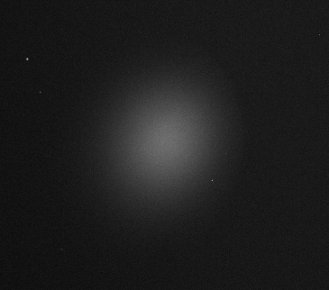
\includegraphics{fourier-020.jpg}};
  \draw [very thick, ->] (5.65,4.1) to [out=80, in=-10] (example.east);
\end{tikzpicture}

  \caption[Measured Fourier plane electron beam size and yield vs incident laser pulse energy on gold photocathode]{
    Measured Fourier plane electron beam size (HWe$^{-1}$M; squares) and electron yield (circles) as a function of the incident $\sim$200fs, 523nm laser pulse energy for the 300nm-thick gold photocathode.
    The electron yield is proportional to the square of laser pulse energy (solid line) and the dependence of the beam size with the laser pulse energy fits that predicted by a zero free parameter electron heating model (solid line; dashed lines represent $\pm$10\% error in the laser spot size).
    A representative raw Fourier plane beam image is also shown.
  }
  \label{fig:gold-emission}
\end{figure}

To verify the efficacy of the experimental technique (see Section \ref{sec:photocathode-method}) for these purposes, we monitored the momentum distribution (Fourier plane spot size) for electrons emitted by 2PTE from gold using the $\sim$200fs green (523nm) $p$-polarized laser pulses.
Due to the 60$^{\circ}$ angle of incidence, the circular laser beam is focused by the 30cm focal length lens to an elliptical 50x100$\mu$m (half-width 1/e maximum (HWe$^{-1}$M) of the field) spot size on the photocathode surface.
The results, the measured Fourier plane beam size and electron yield, are displayed in \ref{fig:gold-emission} as a function of the incident laser pulse energy, corrected to account for 10\% optical loss (mainly from the uncoated vacuum system windows).

The quadratic dependence of the electron yield on pulse energy clearly indicates a two-photon emission process.
This is expected since an excitation energy of two green photons ($\hbar \omega$ = 2.37eV) will be required to overcome the reported $\phi$ = 4.69eV effective work function of a thick gold film contaminated with adsorbed water \cite{monjushiro_ultraviolet_1991} or ensure that at least the tail of the electron Fermi distribution has sufficient energy to overcome the 5.1($\pm$0.1)eV work function of a clean Au surface \cite{eastman_photoelectric_1970}.
Moreover, when $2\hbar \omega \approx \phi$, the dependence of the yield on the square of the electron's excess energy above the work function \cite{monjushiro_ultraviolet_1991} ensures that predominantly only the high energy (Boltzmann) tail of the Fermi distribution contributes to the emission.
Consequently, the observed increase in $\Delta p_x$ with incident pulse energy must be due to a heating effect; specifically, laser heating of the free electron Fermi gas as two-photon excitation is instantaneous and the $\sim$200fs green laser pulse duration excludes any coupling to the lattice which occurs on the time scale of a few picoseconds \cite{chen_semiclassical_2006}.
The solid line in \ref{fig:gold-emission} is the predicted variation derived using a simple zero free parameter model of this effect.
Using the known optical properties of gold \cite{johnson_optical_1972}, which give a reflectance $R_p$ = 0.53 and an absorption depth of 20nm, and the temperature-dependent heat capacity of a free electron Fermi gas, the model evaluates the average temperature of the laser-heated electron gas that may be two-photon excited assuming that only electrons within a few nanometers of the surface can be emitted, as the mean free path for electrons in Au is $\sim$4nm \cite{seah_quantitative_1979}.
This average electron temperature $T_e$ is then used in the AG model simulation of the experiment (\ref{fig:transverse-measurement}) to determine the expected Fourier plane spot size on the YAG scintillator; that is, using an initial $\Delta p_x = \sqrt{m_0 k_B T_e}$.  The dashed lines indicate the expected trends for a $\pm$10\% error in the laser spot size $\Delta x_0$ incident on the gold cathode surface.
The close agreement between the data and the simulation strongly supports our interpretation of the emission mechanism and, as expected, that the effective mass of a free electron in Au is equal to the rest mass $m_0$\cite{johnson_optical_1972}.
